\documentclass[a4paper]{article}
\usepackage{enumitem, amsmath, gensymb, graphicx, caption, amssymb, geometry, fancyhdr, arydshln, adjustbox}

\geometry{left=1in, right=1in, top=1in, bottom=1in}
\pagestyle{fancy}

\newcommand{\myName}{\textbf{Shantanu Ghodgaonkar}\\\textit{Univ ID}: N11344563\\\textit{Net ID}: sng8399\\\textit{Ph.No.}: +1 (929) 922-0614}
\newlist{qalist}{description}{1}
\setlist[qalist]{style=unboxed,leftmargin=0.5cm,labelwidth=2.5cm}


\title{Homework 2 Answers : ROB-GY 6003}
\author{\myName}
\date{\today}

\fancyhead{} % Clear existing header settings 
\fancyhead[L]{\today}
\fancyhead[R]{N11344563}


\begin{document}
	
	\begin{titlepage}
	    \centering
	    \vspace{2cm}
	    \Huge\textbf{Foundations of Robotics \\ ROB-GY 6003 \\ Homework 2 Answers}
	    \vspace{1cm}
	    \\ \Large \today
	    \vfill 
	    \Large \myName
	\end{titlepage}
	
	\begin{qalist}			
		\item[Question: 3.1] \setcounter{equation}{0} %15
		\item[Answer:] Consider below Figure~\ref{fig:3Rarm} \\
			\begin{minipage}{\linewidth}
				\vspace{0.5cm}
				\centering
				\fbox{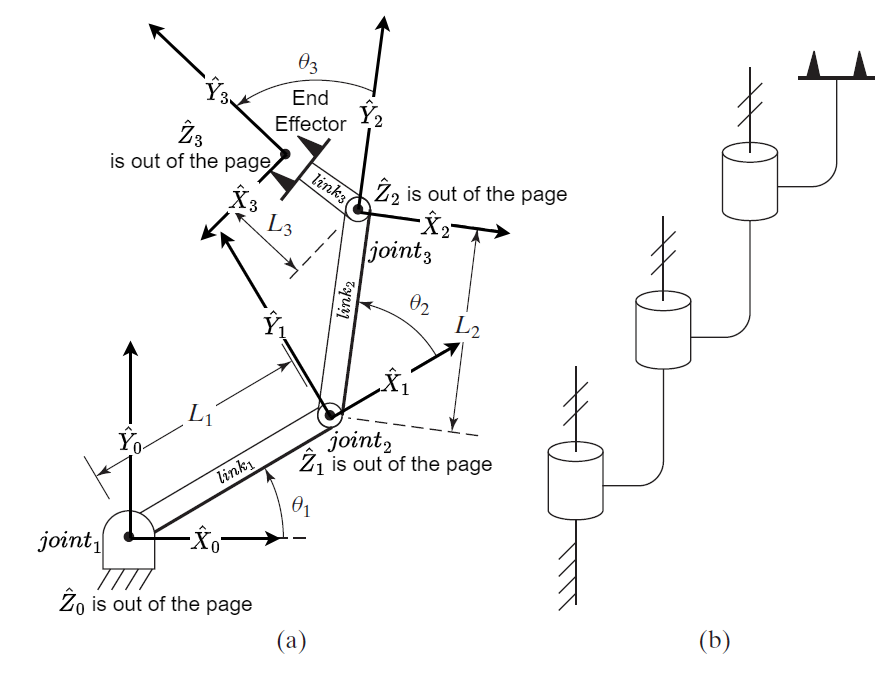
\includegraphics[width=0.5\textwidth]{q3_1.png}}
				\captionof{figure}{A three-link planar arm. On the right, we show the same manipulator by means of a simple schematic notation. Hash marks on the axes indicate that they are mutually parallel.}
				\label{fig:3Rarm}
				\vspace{0.5cm}
			\end{minipage}
			Frames have been attached to each of the \textit{joints} and the \textit{end effector}. 
			We shall now construct the DH Parameter table for this - \\
			\begin{minipage}{\linewidth}
				\vspace{0.5cm}
				\centering
				\begin{tabular}{|c|c|c|c|c|}
					\hline
					${joint}_{i}$ & ${\theta}_{i}$ & ${d}_{i}$ & ${a}_{i}$ & ${\alpha}_{i}$\\
					\hline \hline
					${joint}_{1}$ Revolute & ${\theta}_{1} + {q}_{1}$ & $0$ & ${L}_{1}$ & $0 $\\
					\hline
					${joint}_{2}$ Revolute & ${\theta}_{2} + {q}_{2}$ & $0$ & ${L}_{2}$ & $0$\\
					\hline
					${joint}_{3}$ Revolute& ${\theta}_{3} + {q}_{3}$ & $0$ & ${L}_{3}$ & $0 $\\
					\hline
				\end{tabular}
				\vspace{0.5cm}
			\end{minipage}	
			
		\item[Question: 3.4] \setcounter{equation}{0} %22
		\item[Answer:] Consider below Figure~\ref{fig:q3_4} \\
			\begin{minipage}{\linewidth}
				\vspace{0.5cm}
				\centering
				\fbox{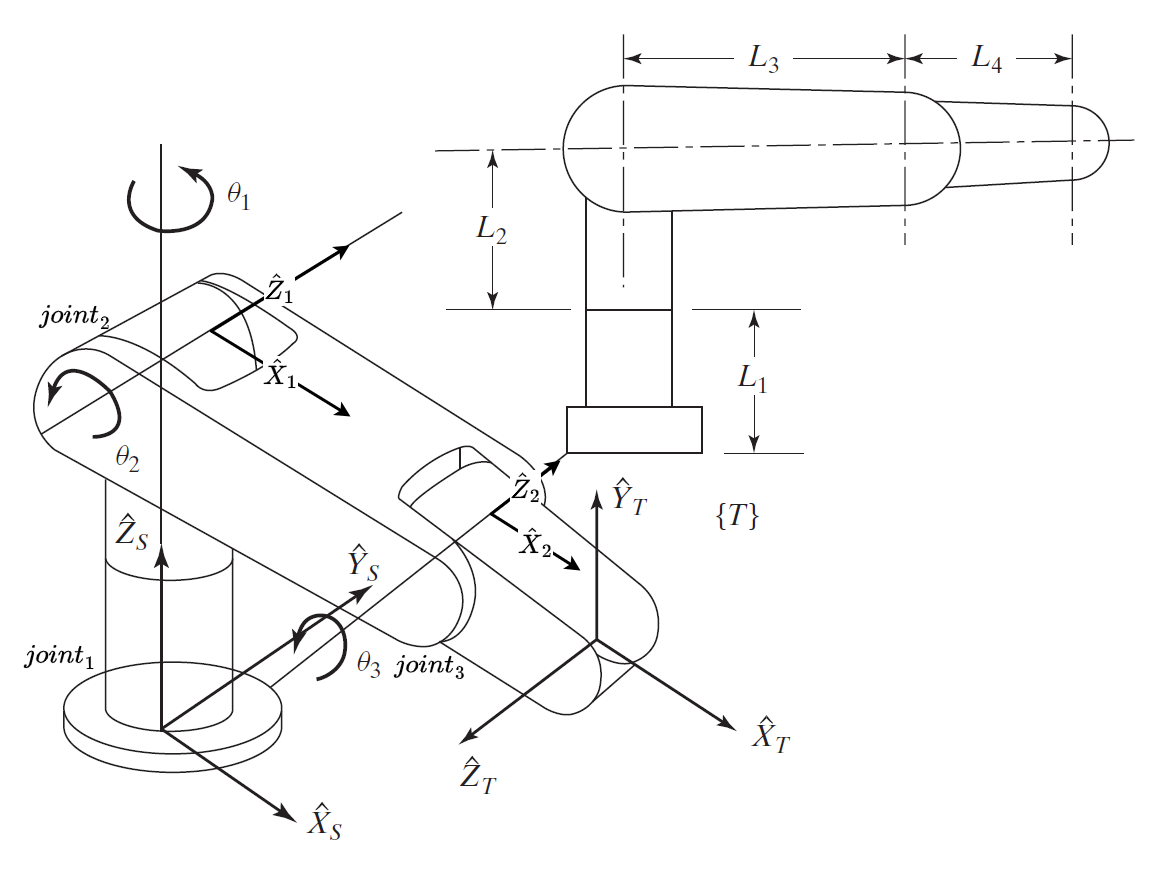
\includegraphics[width=0.5\textwidth]{q3_4.png}}
				\captionof{figure}{Two views of a $3R$ manipulator}
				\label{fig:q3_4}
				\vspace{0.5cm}
			\end{minipage}
			Frames were previously attached to ${joint}_{1}$ the \textit{end effector}. Frames have now been attached to ${joint}_{2}$ and ${joint}_{3}$.
			We shall now construct the DH Parameter table for this - \\
			\begin{minipage}{\linewidth}
				\vspace{0.5cm}
				\centering
				\begin{tabular}{|c|c|c|c|c|}
					\hline
					${joint}_{i}$ & ${\theta}_{i}$ & ${d}_{i}$ & ${a}_{i}$ & ${\alpha}_{i}$\\
					\hline \hline
					${joint}_{1}$ Revolute & $0 + {q}_{1}$ & ${L}_{1} + {L}_{2}$ & $0$ & $0 $\\
					\hline
					${joint}_{2}$ Revolute & $0 + {q}_{2}$ & $0$ & ${L}_{3}$ & $\frac{\pi}{2}$\\
					\hline
					${joint}_{3}$ Revolute & $0 + {q}_{3}$ & $0$ & ${L}_{4}$ & $0 $\\
					\hline
				\end{tabular}
				\vspace{0.5cm}
			\end{minipage}		
			We shall now find the transformation matrices ${}^{S}_{1}T$, ${}^{1}_{2}T$ and ${}^{2}_{T}T$ by applying the generalised equation,
			\begin{equation}
				{}^{i-1}_{i}T = 
				\begin{bmatrix}
					\cos{\theta}_{i} & -\cos{\alpha}_{i}\sin{\theta}_{i} & \sin{\alpha}_{i}\sin{\theta}_{i} & {a}_{i}\cos{\theta}_{i} \\
					\sin{\theta}_{i} & \cos{\alpha}_{i}\cos{\theta}_{i} & -\sin{\alpha}_{i}\cos{\theta}_{i} & {a}_{i}\sin{\theta}_{i} \\
					0 & \sin{\alpha}_{i} & \cos{\alpha}_{i} & {d}_{i} \\
					0 & 0 & 0 & 1
				\end{bmatrix}
			\end{equation}
	
			\begin{equation}
				\Rightarrow {}^{S}_{1}T = 
				\begin{bmatrix}
					\cos{q}_{1} & -\sin{q}_{1} & 0 & 0 \\
					\sin{q}_{1} & \cos{q}_{1} & 0 & 0 \\
					0 & 0 & 1 & ({L}_{1} + {L}_{2}) \\
					0 & 0 & 0 & 1
				\end{bmatrix}
			\end{equation}
			
			\begin{equation}
				\Rightarrow {}^{1}_{2}T = 
				\begin{bmatrix}
					\cos{q}_{2} & 0 & \sin{q}_{2} & {L}_{3}\cos{q}_{2} \\
					\sin{q}_{2} & 0 & -\cos{q}_{2} & {L}_{3}\sin{q}_{2} \\
					0 & 1 & 0 & 0 \\
					0 & 0 & 0 & 1
				\end{bmatrix}
			\end{equation}
			
			\begin{equation}
				\Rightarrow {}^{2}_{T}T = 
				\begin{bmatrix}
					\cos{q}_{3} & -\sin{q}_{3} & 0 & {L}_{4}\cos{q}_{3} \\
					\sin{q}_{3} & \cos{q}_{3} & 0 & {L}_{4}\sin{q}_{3} \\
					0 & 0 & 1 & 0 \\
					0 & 0 & 0 & 1
				\end{bmatrix}
			\end{equation}
		
		\item[Question: 3.8] \setcounter{equation}{0} %13
		\item[Answer:] Consider below Figure~\ref{fig:q3_8} \\
			\begin{minipage}{\linewidth}
				\vspace{0.5cm}
				\centering
				\fbox{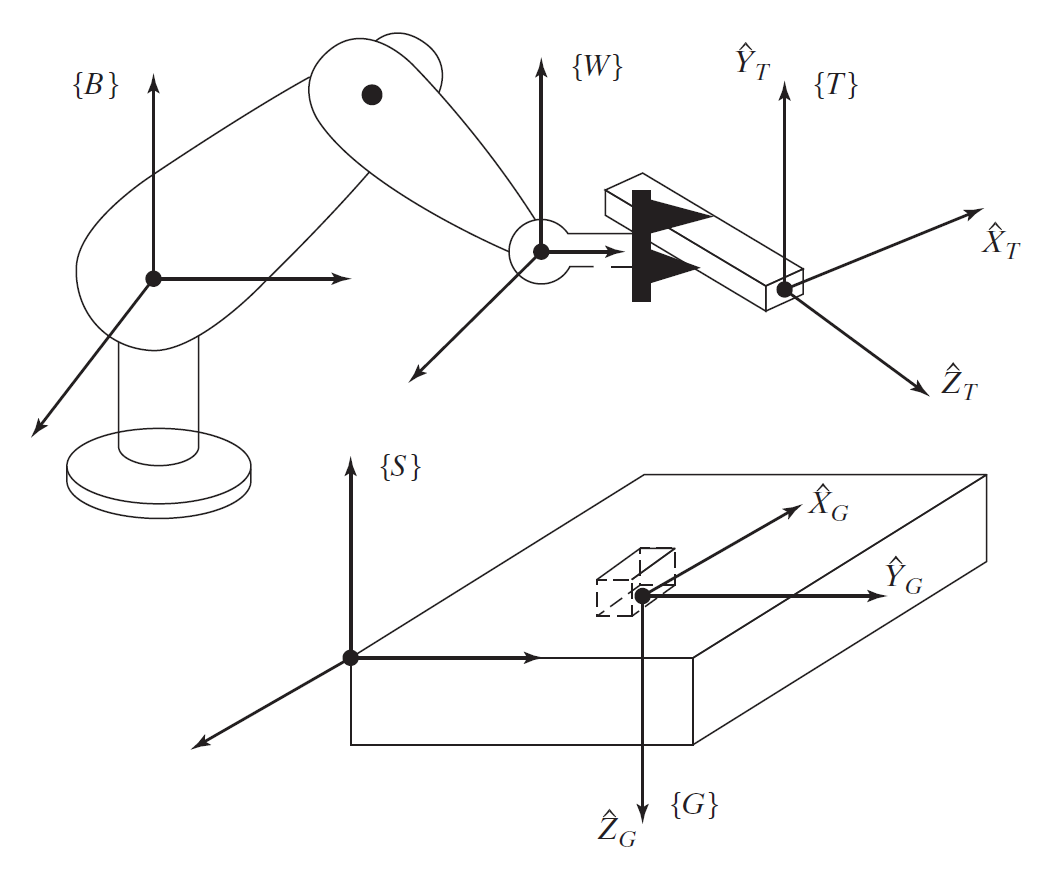
\includegraphics[width=0.6\textwidth]{q3_8.png}}
				\captionof{figure}{Determination of the tool frame}
				\label{fig:q3_8}
				\vspace{0.5cm}
			\end{minipage}
			It is given that the robot feels around with the tool tip until it inserts it into the socket (or Goal). 
			The transformation to this point can be described in two ways. 
			
			Firstly, from the perspective of the robot = ${}^{B}_{W}T \cdot {}^{W}_{T}T$
			
			Secondly, from the perspective of the goal = ${}^{B}_{S}T \cdot {}^{S}_{G}T$
			
			But both of these combination transforms describe the same final position, so,
			
			\[\Rightarrow {}^{B}_{W}T \cdot {}^{W}_{T}T = {}^{B}_{S}T \cdot {}^{S}_{G}T\]
			
			Upon multiplying both sides by ${}^{B}_{W}{T}^{-1}$
			
			\[\Rightarrow {}^{W}_{T}T = {}^{B}_{W}{T}^{-1} \cdot {}^{B}_{S}T \cdot {}^{S}_{G}T\]
		
		\item[Question: 3.12] \setcounter{equation}{0} %08
		\item[Answer:] No. An arbitrary rigid-body transformation requires six parameters. Only in the case that has been described here (according to the D-H Convention) can the rigid-body transformation be expressed with four parameters.
		
		\item[Question: 3.16] \setcounter{equation}{0} %15
		\item[Answer:] The frames are attached as per DH convention given by Spong. See below Figure~\ref{fig:q3_16} -\\
			\begin{minipage}{\linewidth}
				\vspace{0.5cm}
				\centering
				\fbox{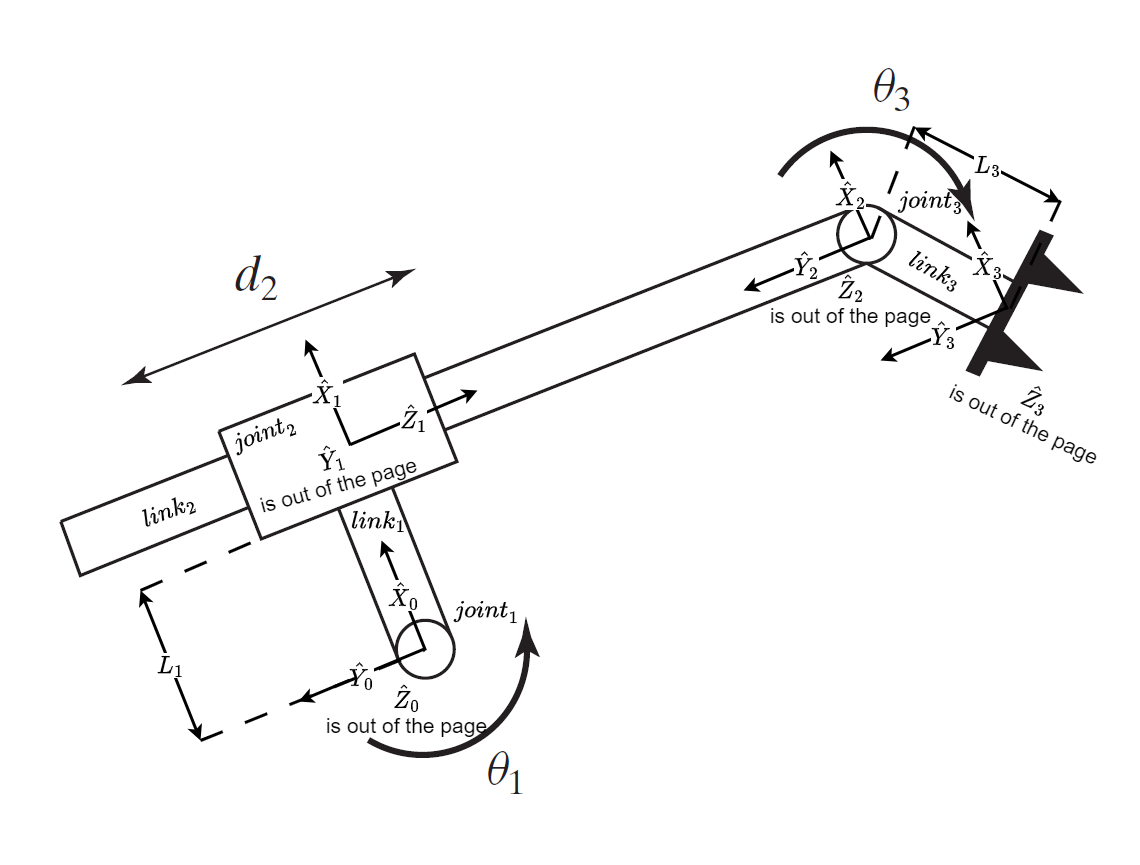
\includegraphics[width=0.6\textwidth]{q3_16.png}}
				\captionof{figure}{The $RPR$ planar robot}
				\label{fig:q3_16}
				\vspace{0.5cm}
			\end{minipage}
			The DH Parameter table is given below - \\ \\
			\begin{minipage}{\linewidth}
				\centering
				\begin{tabular}{|c|c|c|c|c|}
					\hline
					${joint}_{i}$ & ${\theta}_{i}$ & ${d}_{i}$ & ${a}_{i}$ & ${\alpha}_{i}$\\
					\hline
					${joint}_{1}$ Revolute & $0 + {q}_{1}$ & $0$ & ${L}_{1}$ & $\frac{\pi}{2}$\\
					\hline
					${joint}_{2}$ Prismatic & $0$ & ${d}_{2} + {q}_{2}$ & $0$ & $-\frac{\pi}{2}$\\
					\hline
					${joint}_{3}$ Revolute & ${\theta}_{3} + {q}_{3}$ & $0$ & ${L}_{3}$ & $0 $\\
					\hline
				\end{tabular}
			\end{minipage}		
			
		\newpage	
		\item[Question: 3.17] \setcounter{equation}{0} %15
		\item[Answer:] The frames are attached as per DH convention given by Spong. See below Figure~\ref{fig:q3_17} -\\
			\begin{minipage}{\linewidth}
				\vspace{0.5cm}
				\centering
				\fbox{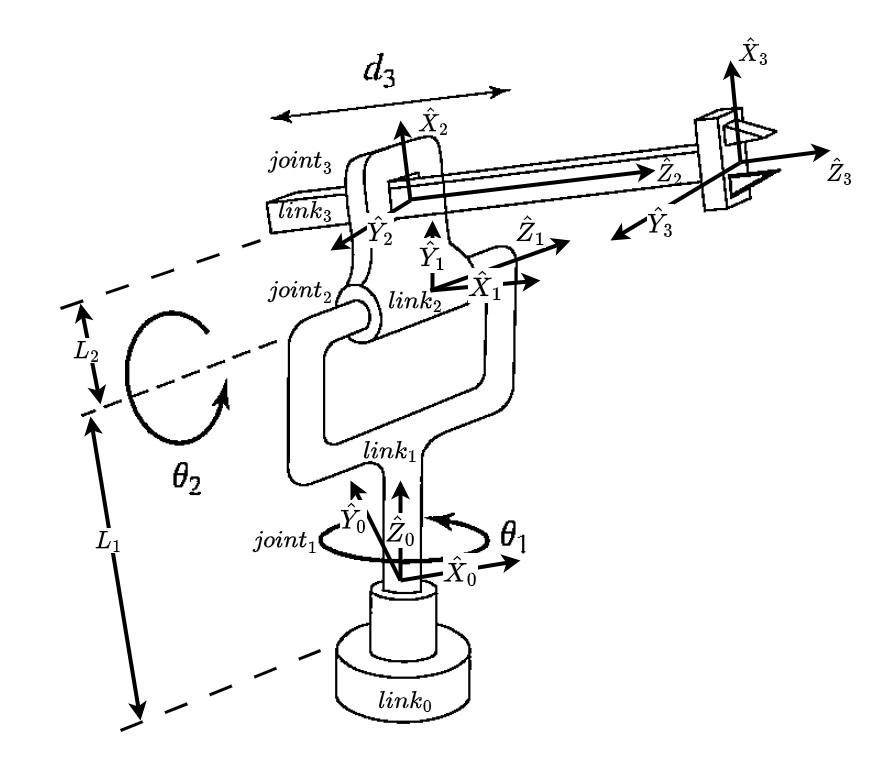
\includegraphics[width=0.6\textwidth]{q3_17.png}}
				\captionof{figure}{Three-link RRP manipulator}
				\label{fig:q3_17}
				\vspace{0.5cm}
			\end{minipage}
			The DH Parameter table is given below - \\ \\
			\begin{minipage}{\linewidth}
				\centering
				\begin{tabular}{|c|c|c|c|c|}
					\hline
					${joint}_{i}$ & ${\theta}_{i}$ & ${d}_{i}$ & ${a}_{i}$ & ${\alpha}_{i}$\\
					\hline
					${joint}_{1}$ Revolute & $0 + {q}_{1}$ & ${L}_{1}$ & $0$ & $-\frac{\pi}{2}$\\
					\hline
					${joint}_{2}$ Revolute & $-\frac{\pi}{2} + {q}_{2}$ & $0$ & ${L}_{2}$ & $-\frac{\pi}{2}$\\
					\hline
					${joint}_{3}$ Prismatic & $0$ & $0 + {q}_{3}$ & $0$ & $0$\\
					\hline
				\end{tabular}
			\end{minipage}	
	\end{qalist}
\end{document}